%%%%%%%%%%%%%%%%%%%%%%%%%%%%%%%%%%%%%%%%%
% Beamer Presentation
% LaTeX Template
% Version 2.0 (March 8, 2022)
%
% This template originates from:
% https://www.LaTeXTemplates.com
%
% Author:
% Vel (vel@latextemplates.com)
%
% License:
% CC BY-NC-SA 4.0 (https://creativecommons.org/licenses/by-nc-sa/4.0/)
%
%%%%%%%%%%%%%%%%%%%%%%%%%%%%%%%%%%%%%%%%%

%----------------------------------------------------------------------------------------
%	PACKAGES AND OTHER DOCUMENT CONFIGURATIONS
%----------------------------------------------------------------------------------------

\documentclass[
11pt, % Set the default font size, options include: 8pt, 9pt, 10pt, 11pt, 12pt, 14pt, 17pt, 20pt
%t, % Uncomment to vertically align all slide content to the top of the slide, rather than the default centered
%aspectratio=169, % Uncomment to set the aspect ratio to a 16:9 ratio which matches the aspect ratio of 1080p and 4K screens and projectors
serif
]{beamer}

\usepackage{color, colortbl}
\definecolor{LightCyan}{rgb}{0.88,1,1}
\usepackage{tikz,pgfplots,float}
\usetikzlibrary {datavisualization.formats.functions}
\usepgfplotslibrary{fillbetween}
\usepgfplotslibrary{groupplots}
\usetikzlibrary{matrix}
\usepackage{xcolor}

\graphicspath{{Images/}{./}} % Specifies where to look for included images (trailing slash required)

\usepackage{booktabs} % Allows the use of \toprule, \midrule and \bottomrule for better rules in tables
\usepackage{amsmath}
\usepackage{amsfonts}
\usepackage{amssymb}

\DeclareMathOperator*{\argmax}{arg\,max}
\DeclareMathOperator*{\argmin}{arg\,min}

\newcommand{\norm}[1]{\left\lVert#1\right\rVert}
\DeclareMathOperator*{\concat}{%
	\mathchoice%
	{\Big\Vert}%
	{\big\Vert}%
	{\Vert}%
	{\Vert}%
}


%----------------------------------------------------------------------------------------
%	SELECT LAYOUT THEME
%----------------------------------------------------------------------------------------

% Beamer comes with a number of default layout themes which change the colors and layouts of slides. Below is a list of all themes available, uncomment each in turn to see what they look like.

%\usetheme{default}
%\usetheme{AnnArbor}
%\usetheme{Antibes}
%\usetheme{Bergen}
%\usetheme{Berkeley}
%\usetheme{Berlin}
%\usetheme{Boadilla}
%\usetheme{CambridgeUS}
%\usetheme{Copenhagen}
%\usetheme{Darmstadt}
%\usetheme{Dresden}
%\usetheme{Frankfurt}
%\usetheme{Goettingen}
%\usetheme{Hannover}
%\usetheme{Ilmenau}
%\usetheme{JuanLesPins}
%\usetheme{Luebeck}
\usetheme{Madrid}
%\usetheme{Malmoe}
%\usetheme{Marburg}
%\usetheme{Montpellier}
%\usetheme{PaloAlto}
%\usetheme{Pittsburgh}
%\usetheme{Rochester}
%\usetheme{Singapore}
%\usetheme{Szeged}
%\usetheme{Warsaw}

%----------------------------------------------------------------------------------------
%	SELECT COLOR THEME
%----------------------------------------------------------------------------------------

% Beamer comes with a number of color themes that can be applied to any layout theme to change its colors. Uncomment each of these in turn to see how they change the colors of your selected layout theme.

%\usecolortheme{albatross}
%\usecolortheme{beaver}
%\usecolortheme{beetle}
%\usecolortheme{crane}
%\usecolortheme{dolphin}
%\usecolortheme{dove}
%\usecolortheme{fly}
%\usecolortheme{lily}
%\usecolortheme{monarca}
%\usecolortheme{seagull}
%\usecolortheme{seahorse}
%\usecolortheme{spruce}
%\usecolortheme{whale}
%\usecolortheme{wolverine}

%----------------------------------------------------------------------------------------
%	SELECT FONT THEME & FONTS
%----------------------------------------------------------------------------------------

% Beamer comes with several font themes to easily change the fonts used in various parts of the presentation. Review the comments beside each one to decide if you would like to use it. Note that additional options can be specified for several of these font themes, consult the beamer documentation for more information.

\usefonttheme{default} % Typeset using the default sans serif font
%\usefonttheme{serif} % Typeset using the default serif font (make sure a sans font isn't being set as the default font if you use this option!)
%\usefonttheme{structurebold} % Typeset important structure text (titles, headlines, footlines, sidebar, etc) in bold
%\usefonttheme{structureitalicserif} % Typeset important structure text (titles, headlines, footlines, sidebar, etc) in italic serif
%\usefonttheme{structuresmallcapsserif} % Typeset important structure text (titles, headlines, footlines, sidebar, etc) in small caps serif

%------------------------------------------------

\usepackage{pifont}
%\usepackage{mathptmx} % Use the Times font for serif text
\usepackage{palatino} % Use the Palatino font for serif text
%\usepackage{pxfonts}
%\renewcommand{\rmdefault}{pxfonts}

%\usepackage{helvet} % Use the Helvetica font for sans serif text
%\usepackage[default]{opensans} % Use the Open Sans font for sans serif text
%\usepackage[default]{FiraSans} % Use the Fira Sans font for sans serif text
%\usepackage[default]{lato} % Use the Lato font for sans serif text

%----------------------------------------------------------------------------------------
%	SELECT INNER THEME
%----------------------------------------------------------------------------------------

% Inner themes change the styling of internal slide elements, for example: bullet points, blocks, bibliography entries, title pages, theorems, etc. Uncomment each theme in turn to see what changes it makes to your presentation.

%\useinnertheme{default}
\useinnertheme{circles}
%\useinnertheme{rectangles}
%\useinnertheme{rounded}
%\useinnertheme{inmargin}

%----------------------------------------------------------------------------------------
%	SELECT OUTER THEME
%----------------------------------------------------------------------------------------

% Outer themes change the overall layout of slides, such as: header and footer lines, sidebars and slide titles. Uncomment each theme in turn to see what changes it makes to your presentation.

%\useoutertheme{default}
%\useoutertheme{infolines}
%\useoutertheme{miniframes}
%\useoutertheme{smoothbars}
%\useoutertheme{sidebar}
%\useoutertheme{split}
%\useoutertheme{shadow}
%\useoutertheme{tree}
%\useoutertheme{smoothtree}

%\setbeamertemplate{footline} % Uncomment this line to remove the footer line in all slides
%\setbeamertemplate{footline}[page number] % Uncomment this line to replace the footer line in all slides with a simple slide count

%\setbeamertemplate{navigation symbols}{} % Uncomment this line to remove the navigation symbols from the bottom of all slides

%----------------------------------------------------------------------------------------
%	PRESENTATION INFORMATION
%----------------------------------------------------------------------------------------

\title[Subquantile Minimization]{Robust Linear Regression by\\ Subquantile Minimization} % The short title in the optional parameter appears at the bottom of every slide, the full title in the main parameter is only on the title page

%\subtitle{Optional Subtitle} % Presentation subtitle, remove this command if a subtitle isn't required

\author[]{Arvind Rathnashyam \and Fatih Orhan \and Josh Myers \and Jake Herman} % Presenter name(s), the optional parameter can contain a shortened version to appear on the bottom of every slide, while the main parameter will appear on the title slide

\institute[Rensselaer Polytechnic Institute]{Rensselaer Polytechnic Institute \\ \smallskip \textit{(rathna, orhanf, myersj5, hermaj2)@rpi.edu}} % Your institution, the optional parameter can be used for the institution shorthand and will appear on the bottom of every slide after author names, while the required parameter is used on the title slide and can include your email address or additional information on separate lines

\date[\today]{ML and Optimization Group U5 \\ \today} % Presentation date or conference/meeting name, the optional parameter can contain a shortened version to appear on the bottom of every slide, while the required parameter value is output to the title slide

%----------------------------------------------------------------------------------------

\begin{document}
	
	%----------------------------------------------------------------------------------------
	%	TITLE SLIDE
	%----------------------------------------------------------------------------------------
	
	\begin{frame}
		\titlepage % Output the title slide, automatically created using the text entered in the PRESENTATION INFORMATION block above
	\end{frame}
	
	%----------------------------------------------------------------------------------------
	%	TABLE OF CONTENTS SLIDE
	%----------------------------------------------------------------------------------------
	
	% The table of contents outputs the sections and subsections that appear in your presentation, specified with the standard \section and \subsection commands. You may either display all sections and subsections on one slide with \tableofcontents, or display each section at a time on subsequent slides with \tableofcontents[pausesections]. The latter is useful if you want to step through each section and mention what you will discuss.
	
	\begin{frame}
		\frametitle{Presentation Overview} % Slide title, remove this command for no title
		
		\tableofcontents % Output the table of contents (all sections on one slide)
		%\tableofcontents[pausesections] % Output the table of contents (break sections up across separate slides)
	\end{frame}
	
	%----------------------------------------------------------------------------------------
	%	PRESENTATION BODY SLIDES
	%----------------------------------------------------------------------------------------
	
	\section{Robust Regression} % Sections are added in order to organize your presentation into discrete blocks, all sections and subsections are automatically output to the table of contents as an overview of the talk but NOT output in the presentation as separate slides
	
	%------------------------------------------------
	
	\subsection{Huber Contamination Model}
	
	\begin{frame}
		\frametitle{Huber Contamination Model}
		
		\begin{Problem}
			The \alert{Huber Contamination Model} is the following:
			\begin{equation*}
				\hat{P} = (1-\varepsilon)P + \varepsilon Q \text{ where } \varepsilon \in (0,0.5)
			\end{equation*}
			where $P$ and $Q$ represent the general linear models
			\begin{equation*}
				\boldsymbol{y}_P = \mathbf{P}\boldsymbol{\beta}_P  + \epsilon_P 
			\end{equation*}
			\begin{equation*}
				\boldsymbol{y}_Q = \mathbf{Q} \boldsymbol{\beta}_Q + \epsilon_Q
			\end{equation*}
			$\boldsymbol{\beta}_P$ and $\boldsymbol{\beta_Q}$ are  oracle regressors and $\epsilon_P$ and $\epsilon_Q$ represent $0$-centered gaussian noise. 
		\end{Problem}
		
		Our goal is to learn a model that learns a good distribution of $P$ from $\hat{P}$
		
		\bigskip % Vertical whitespace
		
	\end{frame}
	
	%------------------------------------------------
	
	\begin{frame}
		\frametitle{Motivation}
		
		\begin{definition}
			In the Robust Statistics literature:\\
			\textbf{Oblivious Noise} is noise generated independent of the target distribution\\
			\textbf{Adaptive Noise} is noise which is generated with knowledge of the target distribution.
		\end{definition}
		\begin{figure}[!t]
			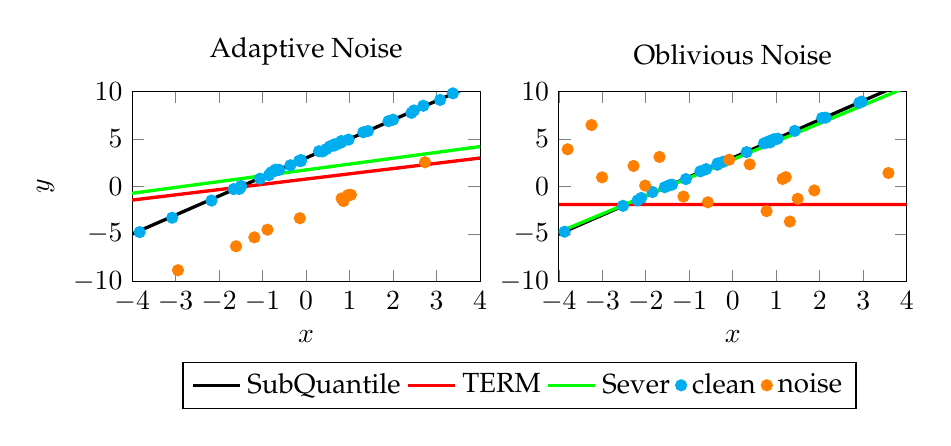
\begin{tikzpicture}
				\begin{groupplot}[group style={group size= 2 by 4},height=4cm,width=6cm,xmax=4,xmin=-4,
					ymin= -10,ymax=10,
					xtick={-4,-3,-2,...,4},
					ytick={-10,-5,0,5,10},]
					\nextgroupplot[title=Adaptive Noise,ylabel={$y$},xlabel={$x$}]
					\coordinate (c1) at (current axis.left of origin);
					\addplot[mark=*,color=cyan,only marks] coordinates{(0.5454756141119426,4.20207144062236) (2.6952740390873733,8.475671650669172) (-0.1612438784423731,2.688323570846449) (1.9998807196500725,7.011477368661404) (0.6573126643085468,4.432503359641061) (0.822541876079238,4.691099695987436) (-1.665736406528514,-0.2771610262088303) (0.2955820690953599,3.6958661148678047) (4.329988449821567,11.633259356797302) (-4.412313203501535,-5.77063957797815) (3.5629538644332275,10.091868592245838) (-0.6175885445775965,1.7473187369931718) (0.8108793561773843,4.772417668204566) (1.4214273053887914,5.818934958869865) (3.081315566792172,9.08926804908307) (-0.12089034451099817,2.6605946971138144) (0.4628376617792958,3.923002461330265) (0.37617729415550505,3.676581100428469) (0.977114787165429,4.918947422974899) (1.314754156260769,5.688804682122404) (-0.36235424331683597,2.2267827837116263) (-0.8007556950385752,1.4886373858967947) (-0.7015664550907283,1.7651694045148667) (-2.1753647987904734,-1.482231084924366) (-1.495574696589605,0.04857682714064265) (-1.0588112744961395,0.8183551891451499) (-3.827119610541674,-4.796523392389788) (-0.8559789159750391,1.1837704089349095) (-0.11761120022533014,2.7730611413376285) (3.3752350984949295,9.778804511993851) (2.4222770389407957,7.727148811092623) (-1.5410032016624133,-0.2633438113497304) (2.480017633230306,7.979402356067379) (0.5911583134769168,4.283748748593926) (-0.71501674964969,1.6324881095139794) (0.6516043112113717,4.294631666773893) (-3.079711134644328,-3.285226613281087) (-1.5088703031224757,-0.08081402676688078) (0.7827672445662932,4.570750601954812) (1.8939059587103262,6.858172766747038)};
					\addplot[mark=*,color=orange,only marks] coordinates{(-2.946629011640607,-8.793723527498958) (0.8607384957406246,-1.538989556510056) (-1.1903001477494382,-5.345751610044574) (1.0305878148541996,-0.8812658035679226) (2.7345343942849927,2.5442143953062244) (-1.6113746066635852,-6.284678207630399) (-0.8883952236652384,-4.5410943399901775) (0.8157297797465353,-1.2566730413348421) (0.9642301396642339,-0.9032576567416104) (-0.14448993411816005,-3.334946134068381)};
					\addplot[domain=-5:5,samples=120,color=black,very thick] {1.99804993*x+2.99972117} ;
					\addplot[domain=-5:5,samples=120,color=red,very thick] {0.55184722*x+0.77673256} ;
					\addplot[domain=-5:5,samples=120,color=green,very thick] {0.61291924*x+1.73788515} ;
					\nextgroupplot[title=Oblivious Noise,xlabel={$x$},legend to name={IntroLegend},legend style={legend columns=5}]
					\coordinate (c2) at (current axis.right of origin);% I moved this to the upper right corner
					\addplot[domain=-5:5,samples=120,color=black,very thick] {2.00041502*x+3.00091281} ;
					\addlegendentry{SubQuantile}
					\addplot[domain=-5:5,samples=120,color=red,very thick] {0.000166177232*x-1.89493121} ;
					\addlegendentry{TERM}
					\addplot[domain=-5:5,samples=120,color=green,very thick] {1.90359844*x+2.82276139} ;
					\addlegendentry{Sever}
					\addplot[mark=*,color=cyan,only marks] coordinates{(0.788762485297498,4.619409754983769) (-1.8444557076323929,-0.5824544981134812) (-3.8667186653234786,-4.754991283615981) (-1.0770702633013416,0.7722164021812354) (-0.35460032498749144,2.2768627851664966) (-6.0822151692288084,-9.06286764938399) (-1.3972518211012221,0.1885381821988659) (2.9097896507970673,8.788974171667162) (-0.3463437020806441,2.420626808504963) (-2.1062359514012012,-1.2085000641078332) (4.336773668705573,11.632780878244247) (-0.6106102670869219,1.8184898177512854) (2.964822961712252,8.905021515559394) (-1.5637145371389622,-0.07761865537709459) (1.0345144344033383,5.0204590940620575) (2.056356483528722,7.198480210723839) (-0.7446791767339869,1.5853174482562558) (0.9631985535487033,4.9300987804715914) (0.8591431516732644,4.6302171243067765) (2.136527593488855,7.225942702339085) (-0.22230647531299189,2.5877920816746207) (1.4255477338524918,5.833868092502212) (-1.4608390115429133,0.12305693654859831) (0.8455335501589681,4.769483861326801) (-2.1885026970448886,-1.4714423105566306) (0.31837311592194245,3.604291796660203) (-2.5244214783210617,-2.0353095069267404) (0.9463907944621844,4.957203119009067) (0.8146787696108556,4.669681514124957) (0.7171745412553174,4.525279797042462)};
					\addlegendentry{clean}
					\addplot[mark=*,color=orange,only marks] coordinates{(-3.2474795820658593,6.450035960386647) (1.8753826722797218,-0.41858598306318395) (1.4931353198669002,-1.2946095099790276) (-6.390816833283051,0.40645831126308823) (0.39048632994899735,2.323962397589362) (-0.08068388106259215,2.8091622671588747) (1.3134080902531131,-3.6866845075408796) (-0.5728261692279717,-1.6637925896534693) (-3.795620644314326,3.901941933326407) (-2.2805802625691634,2.1567188534369586) (-1.1331317978018236,-1.0620378556289347) (-4.057270733769615,6.22788036393642) (3.580927646622491,1.4134339560728868) (1.1473909216831844,0.7892374536150136) (4.60155271303633,1.1396713973323012) (0.777450139132804,-2.5904275309220073) (1.2193257645912936,0.9783812850138183) (-2.0137550195781966,0.08990758847097716) (-3.0052924293950043,0.9558207339897568) (-1.6843214424199917,3.0989236738078767)};
					\addlegendentry{noise}
				\end{groupplot}
				\coordinate (c3) at ($(c1)!.5!(c2)$);
				\node[below] at (c3 |- current bounding box.south)
				{\pgfplotslegendfromname{IntroLegend}};
			\end{tikzpicture}
			\caption{Sub-Quantile Performance on Adapative Outliers}
			\label{fig:structure-unstructured-noise}
		\end{figure}
		
	\end{frame}
	
	%------------------------------------------------
	
	\subsection{Blocks}
	
	\begin{frame}
		\begin{exampleblock}{Theorem}
			The expected optimal parameters of the corrupted model $\hat{P}$
			\begin{equation*}
				\label{eqn:corrupted-optimal}
				\mathbb{E}\left[\boldsymbol{X}^{\dagger}\boldsymbol{y} \right] = (1-\varepsilon)\boldsymbol{\beta}_P + \varepsilon\boldsymbol{\beta}_Q
			\end{equation*}
			where $\boldsymbol{X}^\dagger \triangleq \left(\boldsymbol{X}^\top\boldsymbol{X}\right)^{-1}\boldsymbol{X}^\top$, i.e. the Moore-Penrose Inverse. 
		\end{exampleblock}
		This theorem motivates our reasoning for optimizing over the Subquantile. We want a method to reduce $\varepsilon$. 
	\end{frame}
	
	\begin{frame}
		\frametitle{Statistical Preliminaries of the Subquantile}
		\begin{enumerate}
			\item 
			The quantile is given as the following:
			\begin{equation*}
				\mathcal{Q}_p = \inf\left\{x \in \mathbb{R}: p \leq F(x)\right\}
			\end{equation*}
			\item 
			Let $\ell$ be the loss functions. We can now define risk as:
			\begin{equation*}
				\mathcal{U} = \mathbb{E}\left[\ell(f(\boldsymbol{x};\boldsymbol{\theta}),y)\right]
			\end{equation*}
			\item 
			The $p$-Quantile of the Empirical Risk is given by:
			\begin{equation*}
				\mathbb{L}_p = \frac{1}{p}\int_0^p \mathcal{Q}_q(\mathcal{U})dq = \mathbb{E}\left[\mathcal{U}|\mathcal{U} \leq \mathcal{Q}_p (\mathcal{U})\right] = \max_{t \in \mathbb{R}}\left\{t - \frac{1}{p}\mathbb{E}\left[(t-\mathcal{U})^+\right]\right\}
			\end{equation*}
			\item 
			For the least squares regression case:
			\begin{equation*}
				\mathbb{L}_p = \max_{t\in\mathbb{R}}\left\{t - \frac{1}{np}\sum_{i=1}^n\left(t - \left(\boldsymbol{\theta}^\top\boldsymbol{x}_i - y_i\right)\right)^+\right\}
			\end{equation*}
		\end{enumerate}
	\end{frame}
	
	%------------------------------------------------
	
	\begin{frame}
		\frametitle{Subquantile Optimization Problem}
		We are know able to define the optimization problem we will solve:
		\begin{equation*}
			\boldsymbol{\theta}_{SM} = \operatorname*{argmin}_{\boldsymbol{\theta} \in \mathbb{R}^d}\max_{t\in\mathbb{R}}\left\{t - \frac{1}{np}\sum_{i=1}^n\left(t - \left(\boldsymbol{\theta}^\top\boldsymbol{x}_i - y_i\right)\right)^+\right\}
		\end{equation*}
		
		The objective function is:
		\begin{equation}
			g(t_{(k)},\boldsymbol{\theta}_{(k)}) = t_k - \frac{1}{np}\sum_{i=1}^{n}\left(t - \left(\boldsymbol{x}_i \boldsymbol{\theta} - y_i\right)\right)^+
		\end{equation}
		
		Algorithm:
		\begin{equation*}
			t_{(k+1)} = \operatorname*{argmax}_{t \in \mathbb{R}}g(t,\boldsymbol{\theta}_{(k)})
		\end{equation*}
		\begin{equation*}
			\boldsymbol{\theta}_{(k+1)} = \boldsymbol{\theta}_{(k)} - \alpha \nabla_{\boldsymbol{\theta}}g(t_{(k+1)}, \boldsymbol{\theta}_k)
		\end{equation*}
		
	\end{frame}
	
	\subsection{Preliminaries}
	
	\begin{frame}
		\begin{lemma}
			\begin{equation*}
				\nabla_{\boldsymbol{\theta}} g(t,\boldsymbol{\theta}_{(k)}) = \frac{1}{np}\sum_{i=1}^{np}2\boldsymbol{x}_i\left(\boldsymbol{\theta}^\top_{(k)}\boldsymbol{x}_i - y_i\right)
			\end{equation*}
			where $\left\{(\boldsymbol{x}_i,y_i)\right\}_{i=1}^{np}$ represent the $np$ points in the dataset with the lowest loss.
		\end{lemma}
		\begin{lemma}
			\begin{equation*}
				\operatorname*{argmax}_{t_{k+1} \in \mathbb{R}}g(t,\boldsymbol{\theta}_{(k)}) = y_{np} 
			\end{equation*}
			where $y_{np}$ represents the $np$th highest loss in the dataset.
		\end{lemma}
		Here we are able to see the true nature of Subquantile Optimization. Each iteration we are optimizing over the points within the lowest $np$ errors.  
	\end{frame}
	
	\begin{frame}
		\frametitle{Optimization}
		\begin{definition}
			$(t^*, \boldsymbol{\theta}^*)$ is a \textbf{Local Nash Equilibrium} of $g$ if there exists $\delta > 0$ such that for any $t$, $\boldsymbol{\theta}$ satisfying $\norm{t - t^*}\leq \delta$ and $\norm{\boldsymbol{\theta} - \boldsymbol{\theta^*}} \leq \delta$
		\end{definition}
		\begin{lemma}
			Any Local Nash Equlibrium satisfies $\nabla_{\boldsymbol{\theta}}g(t_{(k)},\boldsymbol{\theta_{(k)}}) = \boldsymbol{0}$ and $\nabla_{\boldsymbol{t}}g(t_{(k)},\boldsymbol{\theta_{(k)}}) = 0$
		\end{lemma}
		We first give intuition on what it means to be at a Local Nash Equilibrium. It means we have a $\boldsymbol{\theta}$ that gives minimizes ERM over the points within the lowest $np$ errors. 
		
	\end{frame}
	
	\begin{frame}
		\frametitle{General Theory}
		
		\begin{lemma}
			Let $\hat{\boldsymbol{\nu}}$ be the losses of all the data ordered in ascending order. Then it follows:
			\begin{equation}
				\argmax_{t \in \mathbb{R}}g(t,\boldsymbol{\theta}) = \hat{\boldsymbol{\nu}}_{np}
			\end{equation}
		\end{lemma}
		Therefore, in each maximizing step we take the element with the $np$th largest loss as $t_{(k+1)}$. With this choice of $t_{k+1}$ it then follows:
		\begin{lemma}
			The derivative with respect to $\theta$ at the $k$th iteration step is:
			\begin{equation*}
				\nabla_{\boldsymbol{\theta}}g(t_{(k+1)},\boldsymbol{\theta}_{(k)}) = \frac{1}{np}\sum_{i=1}^{np}2\boldsymbol{x}_i^T (\boldsymbol{x}_i \boldsymbol{\theta}_{(k)} - y_i)
			\end{equation*}
			where $\boldsymbol{x_1},\dots,\boldsymbol{x}_{np}$ represent the $np$ points with the lowest squared error.
		\end{lemma}
		
	\end{frame}
	
	\begin{frame}
		\frametitle{Prior Works }
		\begin{itemize}
			\item[\ding{228}]
			\cite{DiakonikolasKKLSS19} Sever computes the gradient of losses in each iteration. This incurs a $\mathcal{O}(dn^2)$ time complexity per iteration. Furthermore, points thrown out in early iterations are not resampled. 
			\item[\ding{228}]
			\cite{bhatia2017} CRR runs in order complexity $\mathcal{O}(d^3 + nd)$. The theoretical guarantees of CRR are given only in the case of Oblivious Noise.
			\item[\ding{228}] 
			Our work computes a $np$ partition of the loss in each iteration. This incurs only a $\mathcal{O}(n)$ time complexity per iteration. Subquantile Minimization is novel in that it resamples points that may not have been in previous Subquantiles.
		\end{itemize}
		
	\end{frame}
	
	
	%------------------------------------------------
	
	\section{Empirical Results}
	
	\subsection{Table}
	
	\begin{frame}
		\frametitle{Drug Discovery}
		
		\begin{table}[!h]
			\centering
			\resizebox{\columnwidth}{!}{
				\begin{tabular}{lcccc}
					\toprule 
					\textbf{Objectives}&\multicolumn{4}{c}{Test RMSE (\texttt{Drug Discovery})}\\                   
					\cmidrule(rl){2-5}
					&$\epsilon = 0.1$& $\epsilon = 0.2$& $\epsilon = 0.3$& $\epsilon = 0.4$\\ 
					\midrule
					ERM  &$1.303_{(0.0665)}$&$1.790_{(0.0849)}$&$2.198_{(0.0645)}$&$2.623_{(0.1010)}$\\
					CRR \cite{bhatia2017}  &$1.079_{(0.0899)}$&$1.125_{(0.0832)}$&$1.385_{(0.1372)}$&$1.725_{(0.1136)}$\\
					STIR \cite{pmlr-v89-mukhoty19a} &$1.087_{(0.1256)}$&$1.167_{(0.0750)}$&$1.403_{(0.0987)}$&$1.668_{(0.1142)}$\\
					Robust Risk \cite{RRM} &$1.176_{(0.1110)}
					$&$1.336_{(0.1882)}$&$1.437_{(0.1723)}$&$1.800_{(0.0820)}$\\
					SMART \cite{https://doi.org/10.48550/arxiv.2206.04777} &$1.094_{(0.1065)}$&$1.323_{(0.0758)}$&$1.578_{(0.0799)}$&$1.984_{(0.2020)}$\\
					TERM \cite{li2020tilted} &$\mathbf{1.029_{(0.0707)}}$&$1.126_{(0.0776)}$&$1.191_{(0.1091)}$&$1.201_{(0.1409)}$\\
					SEVER \cite{DiakonikolasKKLSS19} &$1.043_{(0.0970)}$&$\mathbf{1.067_{(0.0457)}}$&$\mathbf{1.071_{(0.0807)}}$&$\mathbf{1.138_{(0.1162)}}$\\
					Huber \cite{Huber2009} &$1.412_{(0.0474)}$&$1.501_{(0.2918)}$&$2.231_{(0.9054)}$&$2.247_{(1.0399)}$\\
					RANSAC \cite{RANSAC1981} &$1.238_{(0.0529)}$&$1.643_{(0.1331)}$&$2.092_{(0.1935)}$&$2.679_{(0.1365)}$\\
					\rowcolor{LightCyan}
					SubQuantile($p = 1-\epsilon$) &$\mathbf{0.966_{(0.1119)}}$&$\mathbf{1.002_{(0.1025)}}$&$\mathbf{1.010_{(0.0630)}}$&$\mathbf{1.082_{(0.1066)}}$\\
					\midrule 
					Genie ERM &$0.960_{(0.0845)}$&$0.982_{(0.0842)}$&$1.006_{(0.0879)}$&$1.030_{(0.0578)}$\\
					\bottomrule
				\end{tabular}
			}
			\caption{\texttt{Drug Discovery} Dataset. Empirical Risk over $P$ with oblivious noise}
			\label{tab:drug-discovery}
		\end{table}
	\end{frame}
	
	%------------------------------------------------
	
	%------------------------------------------------
	
	\section{Mathematics}
	
	\begin{frame}
		\frametitle{Definitions \& Examples}
		
		\begin{definition}
			A \alert{prime number} is a number that has exactly two divisors.
		\end{definition}
		
		\smallskip % Vertical whitespace
		
		\begin{example}
			\begin{itemize}
				\item 2 is prime (two divisors: 1 and 2).
				\item 3 is prime (two divisors: 1 and 3).
				\item 4 is not prime (\alert{three} divisors: 1, 2, and 4).
			\end{itemize}
		\end{example}
		
		\smallskip % Vertical whitespace
		
		You can also use the \texttt{theorem}, \texttt{lemma}, \texttt{proof} and \texttt{corollary} environments.
	\end{frame}
	
	%------------------------------------------------
	
	\begin{frame}[fragile] % Need to use the fragile option when verbatim is used in the slide
		\frametitle{Verbatim}
		
		\begin{example}[Theorem Slide Code]
			\begin{verbatim}
				\begin{frame}
					\frametitle{Theorem}
					\begin{theorem}[Mass--energy equivalence]
						$E = mc^2$
					\end{theorem}
			\end{frame}\end{verbatim} % Must be on the same line
		\end{example}
	\end{frame}
	
	%------------------------------------------------
	
	\begin{frame}
		Slide without title.
	\end{frame}
	
	
	\begin{frame} % Use [allowframebreaks] to allow automatic splitting across slides if the content is too long
		\frametitle{References}
		
		\begin{thebibliography}{99} % Beamer does not support BibTeX so references must be inserted manually as below, you may need to use multiple columns and/or reduce the font size further if you have many references
			\footnotesize % Reduce the font size in the bibliography
			
			\bibitem{DiakonikolasKKLSS19}Diakonikolas, I., Kamath, G., Kane, D., Li, J., Steinhardt, J. \& Stewart, A. Sever: A Robust Meta-Algorithm for Stochastic Optimization. {\em Proceedings Of The 36th International Conference On Machine Learning}. pp. 1596-1606 (2019)
			
			\bibitem{bhatia2017}Bhatia, K., Jain, P., Kamalaruban, P. \& Kar, P. Consistent Robust Regression. {\em Advances In Neural Information Processing Systems}. \textbf{30} (2017), https://proceedings.neurips.cc/paper-files/paper/2017/file/e702e51da2c0f5be4dd354bb3e295d37-Paper.pdf
			
			\bibitem{RRM}Osama, M., Zachariah, D. \& Stoica, P. Robust Risk Minimization for Statistical Learning from Corrupted Data. {\em  IEEE Open Journal Of Signal Processing}. \textbf{1} pp. 287-294 (2020)
			
			\bibitem{pmlr-v89-mukhoty19a}Mukhoty, B., Gopakumar, G., Jain, P. \& Kar, P. Globally-convergent Iteratively Reweighted Least Squares for Robust Regression Problems. {\em Proceedings Of The Twenty-Second International Conference On Artificial Intelligence And Statistics}. \textbf{89} pp. 313-322 (2019,4,16), https://proceedings.mlr.press/v89/mukhoty19a.html
						
			\bibitem{https://doi.org/10.48550/arxiv.2206.04777}Awasthi, P., Das, A., Kong, W. \& Sen, R. Trimmed Maximum Likelihood Estimation for Robust Learning in Generalized Linear Models. (arXiv,2022), https://arxiv.org/abs/2206.04777
						
			\bibitem{li2020tilted}Li, T., Beirami, A., Sanjabi, M. \& Smith, V. Tilted empirical risk minimization. {\em ArXiv Preprint ArXiv:2007.01162}. (2020)
			
			\bibitem{Huber2009}Huber, P. \& Ronchetti, E. Robust statistics. (Wiley,2009), http://catdir.loc.gov/catdir/toc/ecip0824/2008033283.html
			
			\bibitem{RANSAC1981}Fischler, M. \& Bolles, R. Random Sample Consensus: A Paradigm for Model Fitting with Applications to Image Analysis and Automated Cartography. {\em Commun. ACM}. \textbf{24}, 381-395 (1981,6), https://doi.org/10.1145/358669.358692
			
		\end{thebibliography}
	\end{frame}
	
	%----------------------------------------------------------------------------------------
	%	ACKNOWLEDGMENTS SLIDE
	%----------------------------------------------------------------------------------------
	
	%----------------------------------------------------------------------------------------
	%	CLOSING SLIDE
	%----------------------------------------------------------------------------------------
	
	\begin{frame}[plain] % The optional argument 'plain' hides the headline and footline
		\begin{center}
			{\Huge The End}
			
			\bigskip\bigskip % Vertical whitespace
			
			{\LARGE Questions? Comments?}
		\end{center}
	\end{frame}
	
	%----------------------------------------------------------------------------------------
	
\end{document} 